%!TEX root = practicum2.tex
\Cref{alg:percolation} presents our iterative growth process, the defined function expects three arguments \t{N}, \t{probability} and \t{mask}. Given the size parameter \t{N}, the grid used for the percolation is $(N + 1) \times (N + 1)$, since this causes the grid to have an uneven number of rows and columns its center is always clearly defined as $(N, N)$. The parameter $p \in [0, 1]$ is the probability that a given site in the cluster becomes occupied if it is considered. The \t{mask} is a matrix with $r$ rows and $c$ columns that determines the used connectivity. In general four-connectivity is used. This parameter allows us to empirically determine the influence of the connectivity on the growth of the cluster in \cref{ss:exp:connectivity}.

\begin{figure}
	\centering
	\begin{subfigure}{\columnwidth}
		\centering
		
\includegraphics[width=\textwidth]{./img/fancy_cluster_N20_p5}
		\caption{$N = 20$ and $p = 0.5$}
		\label{fig:method:fin_inf:finite}
	\end{subfigure}
	\begin{subfigure}{\columnwidth}
		\centering
		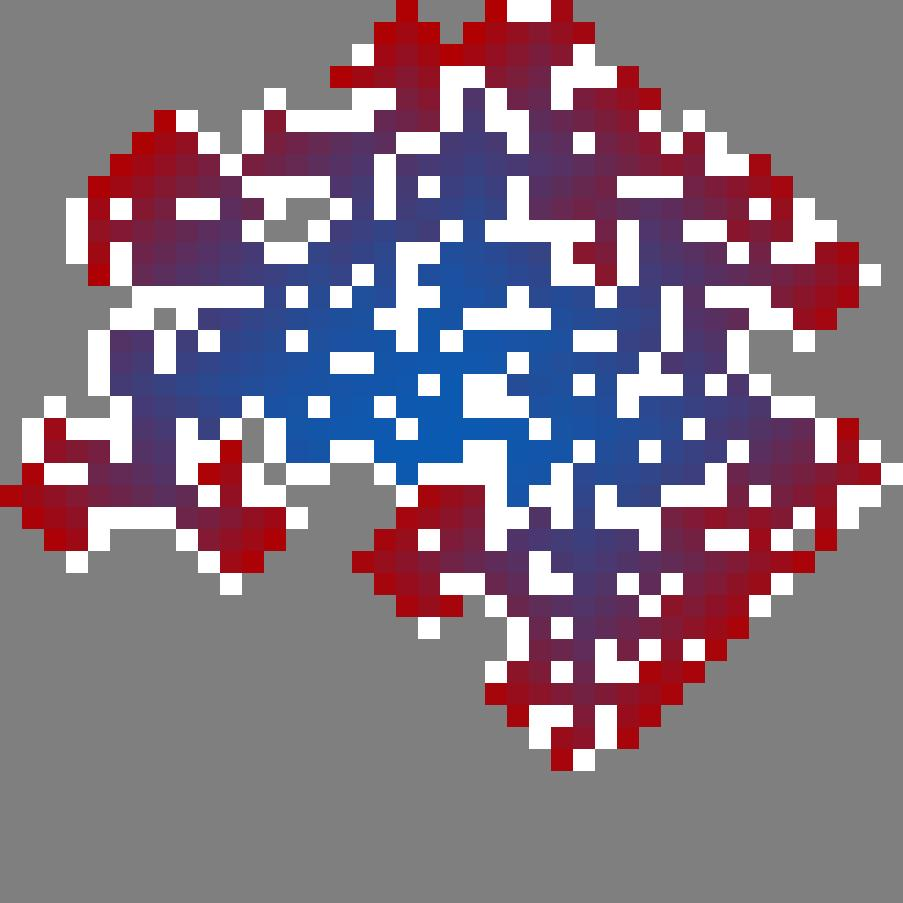
\includegraphics[width=\textwidth]{./img/fancy_cluster_N20_p7}
		\caption{$N = 20$ and $p = 0.7$}
		\label{fig:method:fin_inf:infinite}
	\end{subfigure}	
	\caption{Examples of a finite cluster \subref{fig:method:fin_inf:finite} and percolating cluster \subref{fig:method:fin_inf:infinite}. \todo[inline]{Verwijs naar dit figure. Fix betere plaatjes}}
	\label{fig:method:fin_inf}
\end{figure}

\begin{algorithm}[t]
	\setstretch{1.2}
	\SetAlgoShortEnd
	\DontPrintSemicolon
	\SetKwInOut{Input}{input}\SetKwInOut{Output}{output}
	\Input{	$N$ size\\
			$p$ probability\\
			$mask$ $r \times c$ binary matrix.}
	\Output{$grid$ $(N + 1) \times (N + 1)$ matrix}
	\BlankLine

	$center$ := ($N + 1$, $N + 1$)\; 
	\FuncSty{push($queue$, $center$)}\; 
	$grid$ := \FuncSty{initGrid($N$, $N$)}\; 

	\While{not \FuncSty{isEmpty($queue$)}}{
		$site$ = \FuncSty{pop($queue$)}\; 
		$sites$ = \FuncSty{grow}($grid$, $site$, $mask$, $p$)\; 
		\If{onBorder(site)}{
			\KwSty{break}
		} 
		\FuncSty{push($queue$, $sites$)}\; 
	}\; 
	\caption{\FuncSty{percolation}$(mask, N, p)$\label{alg:percolation}}
\end{algorithm}

% Iteratie
Each iteration we remove the next \t{site} from the queue. We grow this point, using the function \t{grow}. This method considers all neighbors that are connected to \t{site} according to \t{mask}. For each of these neighbors we determine the value $z$, which is randomly sampled from an uniform distribution with the range $[0,1]$. If $z \leq p$ we mark the neighbor site as occupied, otherwise it is marked empty. The method \t{grow} returns the neighbor sites that are occupied, these are added to the queue. 

% Stop conditions
The model stops the growth of the cluster if it is finite or if it is percolating. A cluster is finite if all neighbor sites, according to the connectivity defined by the \t{mask}, of the cluster are marked as empty. In \cref{alg:percolation} we test for this condition via the guard of the loop, if the queue is empty there are no more neighbors to consider, consequently the cluster must be finite. 

A percolating cluster is a cluster that has reached the border of the grid, i.e. if there is a occupied site with row or column number $1$ or $2N + 1$. We test for this condition with the method \t{onBorder}. It should be noted that we only check if a site is on the border of the grid after we have already grown the site. 


